\let\negmedspace\undefined
\let\negthickspace\undefined
\documentclass[journal]{IEEEtran}
\usepackage[a5paper, margin=10mm, onecolumn]{geometry}
%\usepackage{lmodern} % Ensure lmodern is loaded for pdflatex
\usepackage{tfrupee} % Include tfrupee package

\setlength{\headheight}{1cm} % Set the height of the header box
\setlength{\headsep}{0mm}     % Set the distance between the header box and the top of the text

\usepackage{gvv-book}
\usepackage{gvv}
\usepackage{cite}
\usepackage{amsmath,amssymb,amsfonts,amsthm}
\usepackage{algorithmic}
\usepackage{graphicx}
\usepackage{textcomp}
\usepackage{xcolor}
\usepackage{txfonts}
\usepackage{listings}
\usepackage{enumitem}
\usepackage{mathtools}
\usepackage{gensymb}
\usepackage{comment}
\usepackage[breaklinks=true]{hyperref}
\usepackage{tkz-euclide} 
\usepackage{listings}
% \usepackage{gvv}                                        
\def\inputGnumericTable{}                                 
\usepackage[latin1]{inputenc}                                
\usepackage{color}                                            
\usepackage{array}                                            
\usepackage{longtable}                                       
\usepackage{calc}                                             
\usepackage{multirow}                                         
\usepackage{hhline}                                           
\usepackage{ifthen}                                           
\usepackage{lscape}


\renewcommand{\thefigure}{\theenumi}
\renewcommand{\thetable}{\theenumi}
\setlength{\intextsep}{10pt} % Space between text and floats

\numberwithin{equation}{enumi}
\numberwithin{figure}{enumi}
\renewcommand{\thetable}{\theenumi}	

% Marks the beginning of the document
\begin{document}
\bibliographystyle{IEEEtran}

\title{1-1.7-9}
\author{EE24BTECH11049 \\ Patnam Shariq Faraz Muhammed}

% \maketitle
% \newpage
% \bigskip
{\let\newpage\relax\maketitle}

\textbf{QUESTION} \\
	If the points $A = \brak{k + 1, 2k}$, $B = \brak{3k, 2k + 3}$, and $C = \brak{5k - 1, 5k}$ are collinear, then find the value of k.

\textbf{SOLUTION:} \\
\begin{table}[h!]    
  \centering
  \begin{tabular}[12pt]{ |c| c| c|}
\hline
\textbf{Variables} & \textbf{Description} & \textbf{Formula} \\
\hline
$A$ & A point in the 2-D plane whose coordinates are as follows & $\brak{k + 1, 2k}$\\
\hline
$B$ & A point in the 2-D plane whose coordinates are as follows & $\brak{3k, 2k + 3}$\\
\hline
$C$ & A point in the 2-D plane whose coordinates are as follows & $\brak{5k − 1, 5k}$\\
\hline
\end{tabular}

  \caption{Variables Used}
  \label{table: 1.7.9.1}
\end{table}\\
	
        Points $A$, $B$, $C$ are defined to be collinear if
        \begin{align*}
        Rank\myvec{B - A & C - A}^{T}
        \end{align*}
        is equal to 1.

    
        \begin{center}
        \begin{align}
        \myvec{B - A & C - A}^{T} = \myvec{2k-1 & 3 \\ 4k-2 & 3k} 
        \end{align}
        \begin{align}
        \overset{R_2=R_2-2R_1}{\longrightarrow} \myvec{k-1 & 3 \\ 0 & 3k-6}
        \end{align}
        
        For the rank of the matrix to be 1 it should've one non-zero row.\\ 
        make the elements of the $2^{nd}$ row zero.\\
        $\implies 3k-6 = 0$ \\
        $\implies k = 2$ \\
        \end{center}
        
        \begin{figure}[ht]
        \centering
        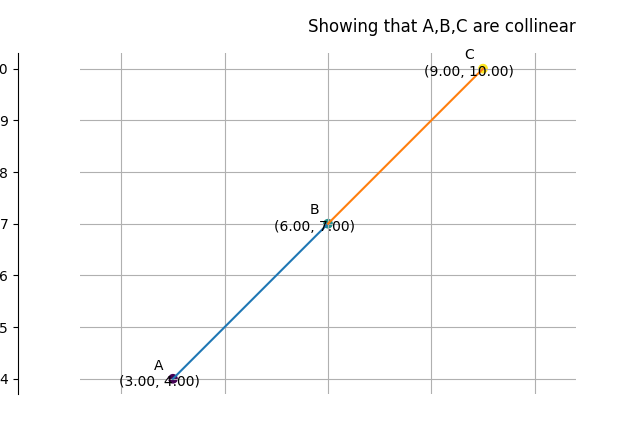
\includegraphics[width=0.7\linewidth]{figs/fig.png}
        \caption{}
        \label{graph}
    	\end{figure}

\end{document}
